\section{Обзор литературы}

Задача поиска путей с контекстно-свободными ограничениями (она же CFPQ) была сформулирована Михалисом Яннакакисом ещё в 1990 году~\cite{Yannakakis1990} в применении к запросам к декларативному языку Datalog~\cite{DatalogWiki, Ceri1989}, textit{но эта идея не была особо развита}.

В последнее десятилетие интерес к задаче \textit{вспыхнул с новой силой} в контексте запросов к RDF (Resource Description Framework)~\cite{RDF}\footnote{Среда описания ресурса}~--- графовой модели представления данных в сети, разработанной W3C (World Wide Web Consortium)\footnote{Консорциум Всемирной паутины}. RDF хранит объекты (ресурсы) и утверждения об их связях (тройки <<субъект~--- предикат~--- объект>>). Чаще всего для работы с данными, представленными в RDF, используют язык запросов SPARQL~\cite{SPARQL}. Однако SPARQL позволяет осуществлять только запросы, представленные в виде регулярных выражений, тогда как некоторые интересные запросы (такие как \textit{same-generation queries}\footnote{Запросы поиска объектов, находящихся на одном уровне иерархии}~\cite{Abiteboul1995}) могут быть выражены только в терминах контекстно-свободных языков.

Задача также нашла широкое применение в разных видах статического анализа~\cite{Reps1998} (в это области она более известная под именем задачи контекстно-свободной достижимости или CFL-Reachability), таких как 

\TODO: написать про виды стат анализа..


% Тем более, некоторые из них встречаются на практике чаще остальных~\cite{Kodumal04}. 

% в основном, основанных на разных видах синтаксического анализа

% : алгоритм Репса~\cite{Reps97}, использующий метод, схожий с алгоритмом Кока-Янгера-Касами~\cite{Younger1967},
 % алгоритм Хеллингса~\cite{Hellings15}, использующий аннотированные грамматики, и другие~\cite{Santos18,Azimov18, Medeiros18, Orachev20, Chaudhuri08}. 

 % К сожалению, недавно Кёйперс и др. экспериментально показали~\cite{Kuijpers19}, что текущие методы не достаточно эффективны для использования на практике. Что не удивительно, так как все они имеют асимптотику $\O(n^3)$ (где $n$~--- размер входного графа, а размер грамматики~--- константа), и лучшее ускорение, которого можно добиться, уменьшает время работы лишь в $\O(\log n)$ раз~\cite{Chaudhuri06} (используя метод четырёх русских~\cite{Arlazarov70}). Более того, существует условная нижняя оценка~\cite{Heintze1997,Chatterjee17}, согласно которой не существует комбинаторного\footnote{Этот термин не вполне определен, но можно понимать его как ``не алгебраический''. В частности, комбинаторные алгоритмы не должны использовать деление и вычитание, так те пользуются особенностями алгебраических структур (а именно, существованием обратного)} субкубического\footnote{С временем работы $\O(n^{3 - \eps})$} алгоритма для задачи CFPQ.

\subsection{Решения задачи в общем случае}

За более чем 30 лет было предложено множество алгоритмов для решения задачи CFPQ. 

Большая часть решений реализует идеи различных алгоритмов разбора выражений (парсинга). Так, алгоритм Мельски и Репса~\cite{Reps97} использует тот же подход, что и алгоритм Кока-Янгера-Касами~\cite{Younger1967} парсинга КС-языков: приведение грамматики к нормальной форме Хомского~\cite{Chomsky1957} и подсчёт динамического программирования~--- и имеет ту же асимптотику $\O(|V|^3 |N|^3)$, где $|V|$~--- число вершин в графе, $|N|$~--- число нетерминалов входной грамматики.

Алгоритм Григорьева и Рогозиной, основан на обобщённом нисходящем синтаксическом анализе\footnote{Top-down parsing}~--- GLL~\cite{Scott10} парсинге, и работает за $\O(|V|^3 \max\limits{v \in V} (deg^{+}(v)))$. Алгоритм Медейроса и др.~\cite{Medeiros18} также основан на нисходящем синтаксическом анализе~--- LL парсинге, но имеет время работы $\O(|V|^3 |P|)$, где $|P|$~--- число продукций входной грамматики.

Алгоритм Сантоса и др.~\cite{Santos18} основан на восходящем синтаксическом анализе\footnote{Bottom-up parsing}~--- LR(1) парсинге~\cite{Aho07}. 

Но есть и другие подходы. 
Например, в своей работе Азимов и Григорьев~\cite{Azimov18} сводят задачу CFPQ к транзитивному замыканию матриц (по аналогии с решением Валианта~\cite{Valiant1975} задачи распознавания КС-языков). Преимущество этого алгоритма в том, что он использует операции над матрицами, которые могут быть соптимизированы с использованием GPGPU\footnote{General-purpose computing on graphics processing units~--- техника использования графического процессора для неграфических целей (математических вычислений)}

% $\O(n^3 k^3 / \log n)$ \cite{Chaudhuri08}
% Алгоритм \cite{Reps97}, к которому применили метод 4 русских

\TODO: Дописать

\subsection{Решения задачи в частных случаях}

\TODO: Всё тут переписать

Понятно, что для решения практических задач далеко не всегда нужна CFPQ в общем случае. Чаще всего для каждой конкретной задачи нужна конкретная КС грамматика, а иногда ещё и понятны ограничения на тип графа.

Пользуясь этой информацией (ограничениями на тип грамматики и графа) можно конструировать частные и потому более быстрые решения. Этим уже занимались, сейчас мы выпишем всё, что на текущий момент известно:

\begin{enumerate}
    \item Язык Дика $\O(n^3 k)$ \cite{Kodumal04}

    Просто применить алгоритм Репса \cite{Reps97} и нормально оценить время работы.

    \item Язык Дика (почти) $\O(n^3)$ \cite{Rehof01}

    Ещё более точный анализ алгоритм Репса \cite{Reps97}, учитывающий, что построенный (для конкретного анализа) граф содержит константное число скобок

    \item Язык Дика на одном типе скобок $D_1$ $\O(n^{\omega} \log^2 n)$ \cite{Mathiasen21}

    Ищем bell-shaped пути: удваиваем рёбра, ищем пути с серединкой из bell-shaped пути поменьше (так $\log n^2$ раз).

    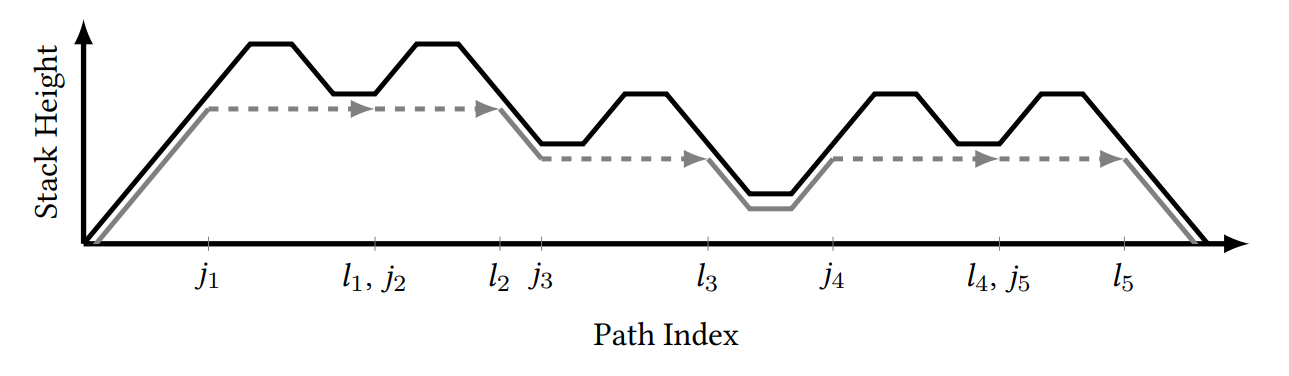
\includegraphics[width=0.75\linewidth]{img/dyck1_path.png}

    Сжимаем bell-shaped пути в $\eps$-рёбра. Снова ищем и снова сжимаем. После каждого сжимания мы убираем все локальные максимумы. Чем больше был максимум, тем длиннее $\eps$-ребро. Хуже всего, когда все новые рёбра длины 2. В любом случае путь становится короче хотя бы в 2 раза, так что таких итераций потребуется не более $\log n^2$ (есть лемма, что найдётся путь длины не более $\O(n^2)$). 

    \item Двунаправленные графы и язык Дика

    Существует несколько частных решений для задачи Диковой достижимости на двунаправленных графах:

    \begin{itemize}
        \item Деревья \cite{Yuan09}

        $\O(n \log n \log k)$~--- центроиды + внутри что-то идейное

        \item Общий случай \cite{Chatterjee17}

        Решение основано на двух фактах. Первый: в двунаправленном графе формируются компоненты Диковой достижимости. Второй: если есть две вершины $u, v$ и компонента Диковой достижимости $C$, такие что $u \xrightarrow{\alpha_i} C$ и $v \xrightarrow{\alpha_i} C$, то $u$ и $v$ тоже лежат в одной компоненте Диковой достижимости. 

        Пользуясь этими фактами, алгоритм с помощью СНМ'а поддерживает компоненты Диковой достижимости и исходящие из них рёбра, чтобы быстро искать новые пары вершин, принадлежащих одной компоненте.

        Итоговая асимптотика алгоритма $\O(m + n \alpha(n))$.
    \end{itemize}

    \item Interleaved Dyck-reachability

        Алгоритм за $\O(n^7)$ для $D_1 \bigodot D_1$ достижимости на bidirected графах~\cite{Li21}

        \textit{Там $\O(n^7)$, потому что авторы~--- дурачки, не умеют рёбра в графе посчитать}

        \textit{Ну или я дурачок, там одно из двух}

        \textit{Было ещё про это (там, вроде, про один из языков сказали, что он bounded, поэтому можно пересекать с регулярным): 
        \url{https://dl.acm.org/doi/pdf/10.1145/3296979.3192378}}
        \TODO: \textit{надо прочитать, что там пишут...}

    \item Граф-цепочка $\O(n^{\omega})$ \cite{Valiant1975}

        CFPQ на графе-цепочке~--- просто задача КС-распознавания (CF-recognition). А она решается за перемножение булевых матриц \cite{Valiant1975}

    \item Ацикличный граф $\O(n^{\omega})$ \cite{Yannakakis1990}

        Ацикличный граф~--- это почти бамбук (= цепочка), нужно только его потопсорить (и где-то ещё быть аккуратным, я не совсем помню сведение)

    \item Bounded-stack RSM $\O(n^3 k^3 / \log^2)$ \cite{Chaudhuri08}

        RSM, который не уходит в рекурсию (т.е. есть из конца ребра $\xrightarrow{S}$ не достижимо никакое ребро $\xrightarrow{S}$)

        Тут применяется какое-то более хитрое (я ещё не разбиралась) итеративное транзитивное замыкание (что-то с dfs'ом, а потом ещё 4 русских сверху, кажется)

    \item Hierarchical FSM $\O(n^{\omega} k^{\omega})$ \cite{Chaudhuri08}

        RSM, в котором боксы упорядочены (топсорт) и бокс с меньшим номером содержит рёбра только с вызовами боксов с большим номером. Задают регулярный язык, но размер FSM может быть экспоненциальным относительно размера RSM.

        Алгоритм идёт в порядке, обратном топсорту, и считает транзитивное замыкание внутри бокса, чтобы провести все рёбра, которые ему соответствуют.

\end{enumerate}

\subsection{Вычислительная сложность}

\TODO

% https://arxiv.org/pdf/2007.05569.pdf


\subsection{Выводы и результаты по главе}

\TODO